
%% bare_conf.tex
%% V1.4b
%% 2015/08/26
%% by Michael Shell
%% See:
%% http://www.michaelshell.org/
%% for current contact information.
%%
%% This is a skeleton file demonstrating the use of IEEEtran.cls
%% (requires IEEEtran.cls version 1.8b or later) with an IEEE
%% conference paper.
%%
%% Support sites:
%% http://www.michaelshell.org/tex/ieeetran/
%% http://www.ctan.org/pkg/ieeetran
%% and
%% http://www.ieee.org/

%%*************************************************************************
%% Legal Notice:
%% This code is offered as-is without any warranty either expressed or
%% implied; without even the implied warranty of MERCHANTABILITY or
%% FITNESS FOR A PARTICULAR PURPOSE! 
%% User assumes all risk.
%% In no event shall the IEEE or any contributor to this code be liable for
%% any damages or losses, including, but not limited to, incidental,
%% consequential, or any other damages, resulting from the use or misuse
%% of any information contained here.
%%
%% All comments are the opinions of their respective authors and are not
%% necessarily endorsed by the IEEE.
%%
%% This work is distributed under the LaTeX Project Public License (LPPL)
%% ( http://www.latex-project.org/ ) version 1.3, and may be freely used,
%% distributed and modified. A copy of the LPPL, version 1.3, is included
%% in the base LaTeX documentation of all distributions of LaTeX released
%% 2003/12/01 or later.
%% Retain all contribution notices and credits.
%% ** Modified files should be clearly indicated as such, including  **
%% ** renaming them and changing author support contact information. **
%%*************************************************************************


% *** Authors should verify (and, if needed, correct) their LaTeX system  ***
% *** with the testflow diagnostic prior to trusting their LaTeX platform ***
% *** with production work. The IEEE's font choices and paper sizes can   ***
% *** trigger bugs that do not appear when using other class files.       ***                          ***
% The testflow support page is at:
% http://www.michaelshell.org/tex/testflow/



\documentclass[10pt, conference, compsocconf]{IEEEtran}
% Some Computer Society conferences also require the compsoc mode option,
% but others use the standard conference format.
%
% If IEEEtran.cls has not been installed into the LaTeX system files,
% manually specify the path to it like:
% \documentclass[conference]{../sty/IEEEtran}


\usepackage{graphicx}
\usepackage{tikz}
\usepackage{wrapfig}
\usepackage{url}
\usepackage{verse}
\usepackage{listings}
\usepackage[margin=1in]{geometry}
\usepackage{color}

\geometry{b5paper,
top=1.5in,
bottom=1.5in,
left=1in,
right=1in}

\newcommand\TODO[1]{{\color{red}[#1]}}

% Some very useful LaTeX packages include:
% (uncomment the ones you want to load)


% *** MISC UTILITY PACKAGES ***
%
%\usepackage{ifpdf}
% Heiko Oberdiek's ifpdf.sty is very useful if you need conditional
% compilation based on whether the output is pdf or dvi.
% usage:
% \ifpdf
%   % pdf code
% \else
%   % dvi code
% \fi
% The latest version of ifpdf.sty can be obtained from:
% http://www.ctan.org/pkg/ifpdf
% Also, note that IEEEtran.cls V1.7 and later provides a builtin
% \ifCLASSINFOpdf conditional that works the same way.
% When switching from latex to pdflatex and vice-versa, the compiler may
% have to be run twice to clear warning/error messages.






% *** CITATION PACKAGES ***
%
%\usepackage{cite}
% cite.sty was written by Donald Arseneau
% V1.6 and later of IEEEtran pre-defines the format of the cite.sty package
% \cite{} output to follow that of the IEEE. Loading the cite package will
% result in citation numbers being automatically sorted and properly
% "compressed/ranged". e.g., [1], [9], [2], [7], [5], [6] without using
% cite.sty will become [1], [2], [5]--[7], [9] using cite.sty. cite.sty's
% \cite will automatically add leading space, if needed. Use cite.sty's
% noadjust option (cite.sty V3.8 and later) if you want to turn this off
% such as if a citation ever needs to be enclosed in parenthesis.
% cite.sty is already installed on most LaTeX systems. Be sure and use
% version 5.0 (2009-03-20) and later if using hyperref.sty.
% The latest version can be obtained at:
% http://www.ctan.org/pkg/cite
% The documentation is contained in the cite.sty file itself.






% *** GRAPHICS RELATED PACKAGES ***
%
\ifCLASSINFOpdf
  % \usepackage[pdftex]{graphicx}
  % declare the path(s) where your graphic files are
  % \graphicspath{{../pdf/}{../jpeg/}}
  % and their extensions so you won't have to specify these with
  % every instance of \includegraphics
  % \DeclareGraphicsExtensions{.pdf,.jpeg,.png}
\else
  % or other class option (dvipsone, dvipdf, if not using dvips). graphicx
  % will default to the driver specified in the system graphics.cfg if no
  % driver is specified.
  % \usepackage[dvips]{graphicx}
  % declare the path(s) where your graphic files are
  % \graphicspath{{../eps/}}
  % and their extensions so you won't have to specify these with
  % every instance of \includegraphics
  % \DeclareGraphicsExtensions{.eps}
\fi
% graphicx was written by David Carlisle and Sebastian Rahtz. It is
% required if you want graphics, photos, etc. graphicx.sty is already
% installed on most LaTeX systems. The latest version and documentation
% can be obtained at: 
% http://www.ctan.org/pkg/graphicx
% Another good source of documentation is "Using Imported Graphics in
% LaTeX2e" by Keith Reckdahl which can be found at:
% http://www.ctan.org/pkg/epslatex
%
% latex, and pdflatex in dvi mode, support graphics in encapsulated
% postscript (.eps) format. pdflatex in pdf mode supports graphics
% in .pdf, .jpeg, .png and .mps (metapost) formats. Users should ensure
% that all non-photo figures use a vector format (.eps, .pdf, .mps) and
% not a bitmapped formats (.jpeg, .png). The IEEE frowns on bitmapped formats
% which can result in "jaggedy"/blurry rendering of lines and letters as
% well as large increases in file sizes.
%
% You can find documentation about the pdfTeX application at:
% http://www.tug.org/applications/pdftex





% *** MATH PACKAGES ***
%
%\usepackage{amsmath}
% A popular package from the American Mathematical Society that provides
% many useful and powerful commands for dealing with mathematics.
%
% Note that the amsmath package sets \interdisplaylinepenalty to 10000
% thus preventing page breaks from occurring within multiline equations. Use:
%\interdisplaylinepenalty=2500
% after loading amsmath to restore such page breaks as IEEEtran.cls normally
% does. amsmath.sty is already installed on most LaTeX systems. The latest
% version and documentation can be obtained at:
% http://www.ctan.org/pkg/amsmath





% *** SPECIALIZED LIST PACKAGES ***
%
%\usepackage{algorithmic}
% algorithmic.sty was written by Peter Williams and Rogerio Brito.
% This package provides an algorithmic environment fo describing algorithms.
% You can use the algorithmic environment in-text or within a figure
% environment to provide for a floating algorithm. Do NOT use the algorithm
% floating environment provided by algorithm.sty (by the same authors) or
% algorithm2e.sty (by Christophe Fiorio) as the IEEE does not use dedicated
% algorithm float types and packages that provide these will not provide
% correct IEEE style captions. The latest version and documentation of
% algorithmic.sty can be obtained at:
% http://www.ctan.org/pkg/algorithms
% Also of interest may be the (relatively newer and more customizable)
% algorithmicx.sty package by Szasz Janos:
% http://www.ctan.org/pkg/algorithmicx




% *** ALIGNMENT PACKAGES ***
%
%\usepackage{array}
% Frank Mittelbach's and David Carlisle's array.sty patches and improves
% the standard LaTeX2e array and tabular environments to provide better
% appearance and additional user controls. As the default LaTeX2e table
% generation code is lacking to the point of almost being broken with
% respect to the quality of the end results, all users are strongly
% advised to use an enhanced (at the very least that provided by array.sty)
% set of table tools. array.sty is already installed on most systems. The
% latest version and documentation can be obtained at:
% http://www.ctan.org/pkg/array


% IEEEtran contains the IEEEeqnarray family of commands that can be used to
% generate multiline equations as well as matrices, tables, etc., of high
% quality.




% *** SUBFIGURE PACKAGES ***
%\ifCLASSOPTIONcompsoc
%  \usepackage[caption=false,font=normalsize,labelfont=sf,textfont=sf]{subfig}
%\else
%  \usepackage[caption=false,font=footnotesize]{subfig}
%\fi
% subfig.sty, written by Steven Douglas Cochran, is the modern replacement
% for subfigure.sty, the latter of which is no longer maintained and is
% incompatible with some LaTeX packages including fixltx2e. However,
% subfig.sty requires and automatically loads Axel Sommerfeldt's caption.sty
% which will override IEEEtran.cls' handling of captions and this will result
% in non-IEEE style figure/table captions. To prevent this problem, be sure
% and invoke subfig.sty's "caption=false" package option (available since
% subfig.sty version 1.3, 2005/06/28) as this is will preserve IEEEtran.cls
% handling of captions.
% Note that the Computer Society format requires a larger sans serif font
% than the serif footnote size font used in traditional IEEE formatting
% and thus the need to invoke different subfig.sty package options depending
% on whether compsoc mode has been enabled.
%
% The latest version and documentation of subfig.sty can be obtained at:
% http://www.ctan.org/pkg/subfig




% *** FLOAT PACKAGES ***
%
%\usepackage{fixltx2e}
% fixltx2e, the successor to the earlier fix2col.sty, was written by
% Frank Mittelbach and David Carlisle. This package corrects a few problems
% in the LaTeX2e kernel, the most notable of which is that in current
% LaTeX2e releases, the ordering of single and double column floats is not
% guaranteed to be preserved. Thus, an unpatched LaTeX2e can allow a
% single column figure to be placed prior to an earlier double column
% figure.
% Be aware that LaTeX2e kernels dated 2015 and later have fixltx2e.sty's
% corrections already built into the system in which case a warning will
% be issued if an attempt is made to load fixltx2e.sty as it is no longer
% needed.
% The latest version and documentation can be found at:
% http://www.ctan.org/pkg/fixltx2e


%\usepackage{stfloats}
% stfloats.sty was written by Sigitas Tolusis. This package gives LaTeX2e
% the ability to do double column floats at the bottom of the page as well
% as the top. (e.g., "\begin{figure*}[!b]" is not normally possible in
% LaTeX2e). It also provides a command:
%\fnbelowfloat
% to enable the placement of footnotes below bottom floats (the standard
% LaTeX2e kernel puts them above bottom floats). This is an invasive package
% which rewrites many portions of the LaTeX2e float routines. It may not work
% with other packages that modify the LaTeX2e float routines. The latest
% version and documentation can be obtained at:
% http://www.ctan.org/pkg/stfloats
% Do not use the stfloats baselinefloat ability as the IEEE does not allow
% \baselineskip to stretch. Authors submitting work to the IEEE should note
% that the IEEE rarely uses double column equations and that authors should try
% to avoid such use. Do not be tempted to use the cuted.sty or midfloat.sty
% packages (also by Sigitas Tolusis) as the IEEE does not format its papers in
% such ways.
% Do not attempt to use stfloats with fixltx2e as they are incompatible.
% Instead, use Morten Hogholm'a dblfloatfix which combines the features
% of both fixltx2e and stfloats:
%
% \usepackage{dblfloatfix}
% The latest version can be found at:
% http://www.ctan.org/pkg/dblfloatfix




% *** PDF, URL AND HYPERLINK PACKAGES ***
%
%\usepackage{url}
% url.sty was written by Donald Arseneau. It provides better support for
% handling and breaking URLs. url.sty is already installed on most LaTeX
% systems. The latest version and documentation can be obtained at:
% http://www.ctan.org/pkg/url
% Basically, \url{my_url_here}.




% *** Do not adjust lengths that control margins, column widths, etc. ***
% *** Do not use packages that alter fonts (such as pslatex).         ***
% There should be no need to do such things with IEEEtran.cls V1.6 and later.
% (Unless specifically asked to do so by the journal or conference you plan
% to submit to, of course. )
\usepackage{url}

% correct bad hyphenation here
\hyphenation{op-tical net-works semi-conduc-tor}


\begin{document}
%
% paper title
% Titles are generally capitalized except for words such as a, an, and, as,
% at, but, by, for, in, nor, of, on, or, the, to and up, which are usually
% not capitalized unless they are the first or last word of the title.
% Linebreaks \\ can be used within to get better formatting as desired.
% Do not put math or special symbols in the title.
\title{Implementing an Open-access, Data Science\\ Programming Environment for Learners}


% author names and affiliations
% use a multiple column layout for up to three different
% affiliations
\author{\IEEEauthorblockN{Austin Cory Bart\IEEEauthorrefmark{1}, Javier Tibau\IEEEauthorrefmark{1}\IEEEauthorrefmark{2}, Eli Tilevich\IEEEauthorrefmark{1}, Clifford A. Shaffer\IEEEauthorrefmark{1}, Dennis Kafura\IEEEauthorrefmark{1}}
    \IEEEauthorblockA{\IEEEauthorrefmark{1}Computer Science\\
Virginia Tech\\
Blacksburg, Virginia, USA\\
acbart@vt.edu, jtibau@vt.edu, tilevich@vt.edu, shaffer@vt.edu, kafura@vt.edu}
    \IEEEauthorblockA{\IEEEauthorrefmark{2}Escuela Superior Polit\'ecnica del Litoral, ESPOL\\
    Km 30.5 V\'ia Perimetral, Guayaquil, Ecuador\\
}
}

% conference papers do not typically use \thanks and this command
% is locked out in conference mode. If really needed, such as for
% the acknowledgment of grants, issue a \IEEEoverridecommandlockouts
% after \documentclass

% for over three affiliations, or if they all won't fit within the width
% of the page, use this alternative format:
% 
%\author{\IEEEauthorblockN{Michael Shell\IEEEauthorrefmark{1},
%Homer Simpson\IEEEauthorrefmark{2},
%James Kirk\IEEEauthorrefmark{3}, 
%Montgomery Scott\IEEEauthorrefmark{3} and
%Eldon Tyrell\IEEEauthorrefmark{4}}
%\IEEEauthorblockA{\IEEEauthorrefmark{1}School of Electrical and Computer Engineering\\
%Georgia Institute of Technology,
%Atlanta, Georgia 30332--0250\\ Email: see http://www.michaelshell.org/contact.html}
%\IEEEauthorblockA{\IEEEauthorrefmark{2}Twentieth Century Fox, Springfield, USA\\
%Email: homer@thesimpsons.com}
%\IEEEauthorblockA{\IEEEauthorrefmark{3}Starfleet Academy, San Francisco, California 96678-2391\\
%Telephone: (800) 555--1212, Fax: (888) 555--1212}
%\IEEEauthorblockA{\IEEEauthorrefmark{4}Tyrell Inc., 123 Replicant Street, Los Angeles, California 90210--4321}}




% use for special paper notices
%\IEEEspecialpapernotice{(Invited Paper)}




% make the title area
\maketitle

% As a general rule, do not put math, special symbols or citations
% in the abstract
\begin{abstract}
A key retention issue when educating computing novices is ensuring that the frustrations of mastering programming fundamentals do not demotivate students. 
Non-CS majors often struggle to find relevance in traditional computing curricula that tend to either emphasize abstract concepts, focus on non-practical entertainment (e.g., game/animation design), or rely on decontextualized settings.
To assist with these issues, this paper introduces BlockPy (\url{http://www.blockpy.com}), a web-based, open-access Python programming environment that supports introductory programmers in a Data Science context.
It promotes long-term transfer by scaffolding an introduction to textual programming through a block-based programming view, ideal for beginners.
BlockPy is designed for informal learners and formal classes, and provides guiding feedback within interactive programming problems.
The results from a pilot of the initial deployment of BlockPy indicates that the environment addresses many problems faced by novice learners.
\end{abstract}

% no keywords

\begin{IEEEkeywords}
Computer science education; Computer aided instruction; Data analysis; Web services;
\end{IEEEkeywords}


% For peer review papers, you can put extra information on the cover
% page as needed:
% \ifCLASSOPTIONpeerreview
% \begin{center} \bfseries EDICS Category: 3-BBND \end{center}
% \fi
%
% For peerreview papers, this IEEEtran command inserts a page break and
% creates the second title. It will be ignored for other modes.
\IEEEpeerreviewmaketitle

As computing becomes pervasive in our society across fields, working professionals increasingly need some expertise in computing alongside their core domain knowledge.
General education computing curricula at the university level (e.g., ``Computational Thinking'' courses) are scaling, Massively Open Online Courses are flourishing, and a large class of learners are pursuing non-formal learning experiences on their own.
Both these traditional and non-traditional learners often have little experience with computing, low self-efficacy, and are uncertain how computing benefits their long-term career goals.
Not only do they need special scaffolding unique to their ability and motivational level, but they also need fewer barriers in accessing these materials.
Our new tool to better serve this population is BlockPy: an open-access, web-based Python environment for data science that supports learners with guided instruction and an accessible interface (\url{http://www.blockpy.com}).

\textbf{Why Data Science?}
Modern approaches to contextualizing introductory courses have focused on making the experience ``fun'' and ``interesting'', with an emphasis on game design and media computation.
However, student motivation is a complex construct dependent on more than just situational interest; holistic models of motivation suggest that students also need to feel that the material is useful to learn, and that long-term career goals are satisfied~\cite{jones-description}.
Contexts like Media Computation are not always perceived as authentically useful  for non-majors, based on a study by Guzdial et al~\cite{guzdial2006imagineering}.

We suggest that Data Science is a motivating context that can appeal in a different way to students, thanks to the wide-spread need for data processing in other majors.
In a previous work, we have reported on the affordances and impacts of Data Science as a learning context~\cite{sigcse17-corgis}.
Often, students study computing to learn how to manage the dizzying quantities of data being stored and analyzed in a discipline or for a specific self-derived project.
By grounding the content in this context, students can be more easily convinced of the relevance of computing and understand how the materials fit together more clearly.
By aligning the context with students' long-term needs, students also learn skills more relevant to those needs.
Finally, data science as a context naturally lends itself to teaching topics related to structured data, iteration, and other core material, making it a pedagogically valuable context to the CS instructor.

\textbf{Why Python?}
Python has become one of the most popular introductory programming languages~\cite{guo2014python}, thanks to its simple syntax combined with impressive power.
It includes strong support for data science thanks to popular libraries like MatPlotLib.
Python requires little code to accomplish interesting things, so novices are not bogged down with complex syntactical details.
Its wide-spread use in both introductory classes and industry further motivated our choice.

\textbf{Why Blocks?}
Any kind of programming is a challenge to beginners, due to the nature of coding as the ``most powerful, but least usable human-computer interface ever invented''~\cite{koh-ui-programming}.
Block-based languages (such as Scratch and AppInventor) have been shown to mitigate the start-up time for students to begin programming and accomplish tasks~\cite{bbl-Price,WeintropIcer}.
By providing structure and an immediate view into the entire user interface of a language, blocks greatly benefit introductory learners.

\begin{figure*}[ht]
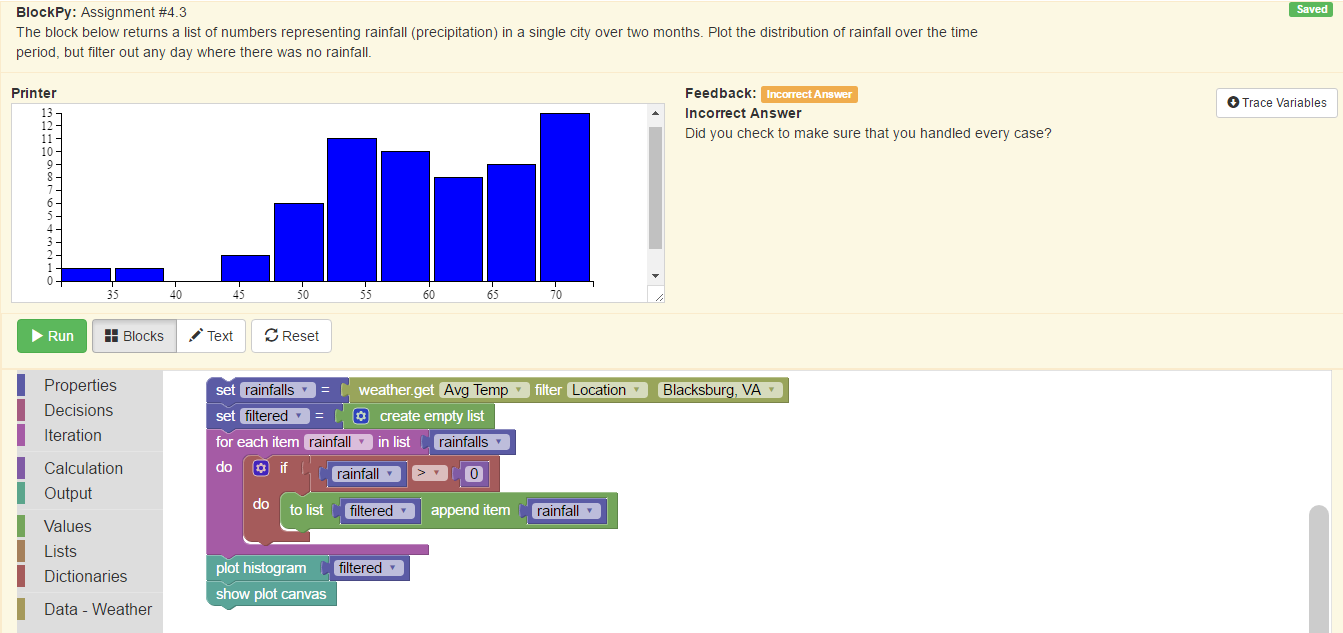
\includegraphics[width=\textwidth]{images/blockpy-interface-2}
\caption{BlockPy in action}
\label{fig-blockpy-full}
\end{figure*}

\textbf{Why Another Python Web Environment?}
There are several environments available today that let students and instructors write Python in the browser, including CodeSkulptor~\cite{CodeSkulptor-Tang}, Pythy~\cite{pythy}, and the Online Python Tutor~\cite{Guo:2013}.
BlockPy stands on the shoulders of giants, integrating features inspired by these environments and introducing novel ones.
But none of these existing Python environments transitions students into textual programming languages.

BlockPy was designed to provide dual support for both block-based and text-based code authoring.
At any time, the student can switch freely between a block-based view of their code and a traditional text-based view.
This powerful feature is inspired by Pencil Code, which uses its own Logo language~\cite{Bau}, and similar implementations have been successful as a fading scaffold for students~\cite{Matsuzawa}.

BlockPy extends Pythy's~\cite{pythy} support for ``assignments'', problems that integrate presentation with assessment.
However, Pythy only supports traditional unit testing to provide students with feedback, while BlockPy provides an API for code analysis and free-form text guidance that instructors can configure to give helpful suggestions to their students.
Furthermore, Pythy has limited support for data science, whereas BlockPy has a rich library of data sources and a MatPlotLib-based plotting API.

CodeSkulptor, Pythy, and BlockPy all use the same internal engine for running Python code (``Skulpt''). 
Although CodeSkulptor has an extensive API for creating user interfaces and games, it provides a non-standard library.
Although suitable for beginners, this library does not aid the transition to serious programming environments.
In BlockPy, the philosophy is to maintain approximate compatibility with real systems.
Instead of a custom plotting API, for instance, we mimic the MatPlotLib interface.

OnlinePythonTutor has proven to be a useful tool for visualizing program state.
However, OPT gives a depth of detail that can overwhelm introductory students (e.g., terminology such as Frames and Objects, which might be foreign to students).
BlockPy's state explorer does not attempt to match OPT's thoroughness, but instead provides a helpful yet simple picture of program state.
Additionally, we avoid OPT's server dependency by relying on Skulpt, which runs in the browser.

\section{BlockPy}

The primary design goals of BlockPy are as follows.

\begin{enumerate}
\item Reduce barriers to learning programming.
\item Promote authenticity by empowering students to complete real-world problems.
\item Promote maturity by faded scaffolds (e.g., transitioning from blocks to text).
\item Minimize the need for help from human instructors.
\end{enumerate}

\subsection{Open-source, Open-access}

The fundamental vision of BlockPy is a highly accessible, web-based platform for anyone to learn how to program.
All code is open-source, and leverages a number of open-source libraries.
There is no registration needed to use the software, although there are features that benefit from free registration, such as managing classrooms.
We provide guided learning materials, to be shared by educators.

The BlockPy editor continuously stores user code as it is entered.
Logs are stored at the keystroke level for future program analysis (described in Section~\ref{PA-description}).
The latest version of the user's code is therefore available between sessions.
When operating in offline mode, the code is stored in the \texttt{LocalStorage} browser object; when the connection is reestablished, synchronization is performed.

\subsection{Python Execution}

The BlockPy system is built to work offline, ideal for places where internet connectivity is unreliable.
Python Code Execution is achieved through a modified instance of the Skulpt JavaScript library.
Skulpt is a full Python parser and compiler, supporting almost all Python language features by generating JavaScript code.
This includes partial support for the rich Python standard library.
The Skulpt execution environment resides entirely within the users' browser, so there is no reliance on an external server beyond the initial page load.

\subsection{Block-based Python}

To support introductory learners as they grapple with Python syntax, the initial interface in BlockPy is block-based, using the popular Blockly JavaScript library.
Language features (iteration, decision, variable assignment and access, etc.) are contained in a toolbox on the left side, from which users drag-and-drop blocks onto a canvas.
BlockPy's block interface only generates syntactically valid Python code, enforced by the ``snapping'' connectors of the blocks (although it is possible to generate semantically incorrect code -- discussed later).
This block interface is synchronized with a text interface; section \ref{MLT-description} describes these two interfaces.

An important question is how many language details should be exposed, and at what rate.
A rarely used feature of \texttt{for} loops in Python is to contain an \texttt{else} clause that is executed upon successful completion of the loop (that is, when it is not prematurely escaped using a \texttt{break} statement).
This advanced language feature is similar to a \texttt{finally} statement with exceptions.
However, if an \texttt{else} clause were made available to beginners first trying to grapple with iteration, it is likely they would confuse the concept with the conditional \texttt{else} clause used in \texttt{if} statements.
Cognitive load is harsh to beginners, and the user interface needs to avoid exposing unnecessary details where possible.
While hiding \texttt{else} bodies in a \texttt{for} loop is a clear case, there are more subtle examples.
It can be difficult to recognize when the learner is ready to use parallel assignment, and therefore should be able to specify multiple variables on the left side of an assignment block.
A block-based language forces a teacher to make important decisions about how to expose language features.
As part of the future work of BlockPy, we are experimenting with exposing language features at different rates, adjustable by the instructor, so the system can expose a progressively more accurate language model.

\subsection{Adaptive Guided Practice}

One of the most powerful features of BlockPy is the interactive, guided feedback feature.
A limitation of programming environments like Snap! is that they are not pedagogically interactive --
students completing an assignment in the system are not guided to success.
The learner must decide when they have completed their program, and whether it meets the specification.
For independent learners outside of a formal learning experience, this requires high levels of self-regulation and meta-cognition.
BlockPy's adaptive elements follow an Expert model; when students run their code, it is checked against instructor-provided logic.
If the student code fails for some reason, they are offered a suggestion.
Correct code gives a green ``Complete'' mark -- we have found that this positive marker has motivating power.

In the Instructor Mode, teachers provide a problem instance.
First, a WYSIWYG rich-text editor edits the problem description, supporting any valid HTML content (e.g., images, links). 
Second, the instructor provides code in special canvases that affect the students' experience.
Instructors write this code using the same text/block interface that students use.
First is the ``starting code'', shown to the student when they begin the problem, avoiding a blank canvas.
The second instructor code defines interactive feedback, which can access the students' code, their final output, and a complete trace of their program's state.
The checking system can declare the code to be correct, or display an HTML string that is rendered as user feedback.
The instructor is free to write whatever logic they want, such as searching for a specific Abstract Syntax Tree (AST) element, testing the outputs on the console, or walking through the programs state to satisfy invariants.
An API for common checks is evolving based on common use cases, such as parsing the program's AST to ensure that they are not calling forbidden built-in Python functions.
We are also exploring interventions an instructor can make beyond rendering textual feedback; perhaps displaying a pop-up dialog with an embedded instructional video, or alerting an instructor to provide Just-In-Time instruction for a particular struggling student.
Finally, we are experimenting with a new system for modeling students' misconceptions related to programming, in order to provide better guidance tuned to students' specific mistakes.

\subsection{Program Analysis for Deeper Learning} \label{PA-description}

BlockPy uses simple program analysis techniques to find both general mistakes that novices make, and problem-specific errors.
For example, beginners often fail to understand the true purpose of certain variables, and incorrectly include them due to mimicking an example.
By performing simple variable liveness analyses, we can identify these variables and raise an error.
Most modern editors feature this kind of analysis, but usually trust that the user has a reason and responds passively; the nature of our learners requires stronger responses.

Since we securely record the history of users' programs and log interface interactions,
we can mine this repository of code to infer common patterns that suggest undesirable learner behavior.
For example, users that frequently move the same blocks without progressing in the problem objectives might be indicative of taking longer on the problem than other users.
Alternatively, students who pick a decision block to complete a problem about iteration might need extra attention.
By proving or disproving such hypotheses, we can improve the automatic feedback of the system and provide more individualized support.

\subsection{LTI Support}

%\begin{figure}
%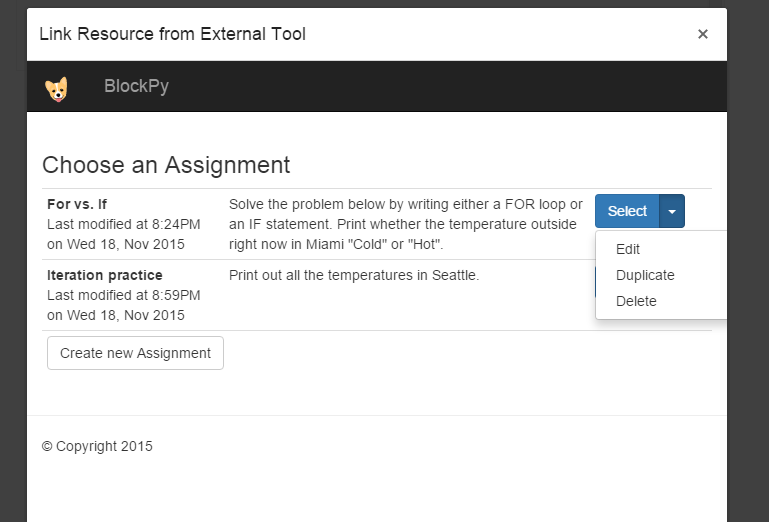
\includegraphics[width=0.5\textwidth]{images/blockpyLTI}
%\caption{Teacher Perspective for Managing BlockPy Assignments}
%\label{fig-lti-teacher}
%\end{figure}

BlockPy supports the LTI (Learning Technology Interoperability) protocol.
This is a mechanism by which instructors can embed questions in their existing course management software (e.g., Canvas, OpenEdX) and receive assignment outcomes (e.g., a grade).

A typical learner uses BlockPy without ever being aware of LTI.
An instructor using the system obtains a secret key and configuration URL that is used within their Learning Management System.
Students on a course website may use BlockPy without registering for a BlockPy account -- the first time they log in through their LMS' provided link, they are invisibly registered in the system with a regular account through additional information from the LMS.
As students complete work, assignment progress is reported back to the LMS.
Instructors use a special interactive menu for managing exercises associated with a course.

\subsection{Data Science Blocks}

BlockPy focuses on Data Science as its primary context, and so we have blocks for working with data.
We support a subset of the popular MatPlotlib library, and extend it with connections to the CORGIS project~\cite{CORGIS}.
The MatPlotLib API, for example, provides a ``plot(list)'' function to create simple line plots.
By mimicking MatPlotLib, students can seamlessly shift to a serious Python programming environment without loss of code. 

The CORGIS (Collection of Real-time, Giant, Interesting, Situated datasets) Project makes motivating datasets available to introductory students through simple programming libraries~\cite{CORGIS}.
These datasets are drawn from many disciplines, resulting in material meant to be universally interesting and relevant.
Currently, BlockPy supports a number of different CORGIS libraries including weather data, earthquake data, United States crime statistics, and a classic book dataset.

\begin{figure}
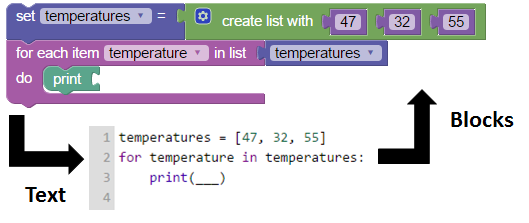
\includegraphics[width=0.5\textwidth]{images/mltExample-2}
\caption{User perspective of block/text transition}
\label{fig-mlt-user}
\end{figure}

\subsection{Mutual Language Translation} \label{MLT-description}

A technical contributions of this project is the mutual language translation between Blockly and Python.
Blockly outputs valid python source code, which can be passed into Skulpt to extract a JSON representation of the Abstract Syntax Tree.
This AST is parsed using our own Py2Block library to generate an XML representation that Blockly can render in the Block View.
Figure~\ref{fig-mlt-user} demonstrates the users' experience.
When a student tries to convert code with disconnected blocks, the generated Python code will be filled in with triple underscores.
These underscores (usually a valid variable name in Python) will trigger a run-time error.

Blockly already supports compilation of its blocks to Python, JavaScript, PHP, and Dart.
However, this multiple language support causes reduced isomorphism---each language has different syntax for their common operations, and it is impossible to create a fully-featured block language with a one-to-one mapping to them all.
For example, JavaScript has no support for parallel assignment, a commonly-used feature in Python, while Python does not have a unary increment operator.
Blockly itself has syntax and vocabulary descended from Logo.

Instead of trying to satisfy multiple languages, we have dropped support for other languages for a more fully-featured mapping to Python.
This requires minor changes that introduce Python-centric syntax details:
function blocks are labeled ``define'', assignment blocks have an ``='' symbol, the ``add item to list'' block is renamed to ``append''.
Blockly has also been extended with new language features, including dictionary access and creation.

Eventually, the interface should offer a complete isomorphic mapping to Python.
However, there are a number of complications to resolve first.
For instance, Python uses square brackets for both list indexing and dictionary access.
There is a strong desire to differentiate between these types of access, visible in the block view as two distinct kinds of blocks (``get ith element of list'' vs. ``get key from dict'' blocks).
However, it is computationally difficult to statically identify the usage of a given pair of brackets-- sophisticated program analysis techniques are needed.

\subsection{Parson's Problems}

Parsons' Problems are a special type of coding exercise where all of the necessary code blocks are present, but disconnected and shuffled.
These kinds of problems scaffold beginners by providing everything they need to complete the problem, reducing many of the barriers to getting started.
BlockPy supports these types of problems with a special ``Parsons Mode'' where top-level blocks are shuffled in the block mode.


% \begin{figure}
% \begin{center}
% 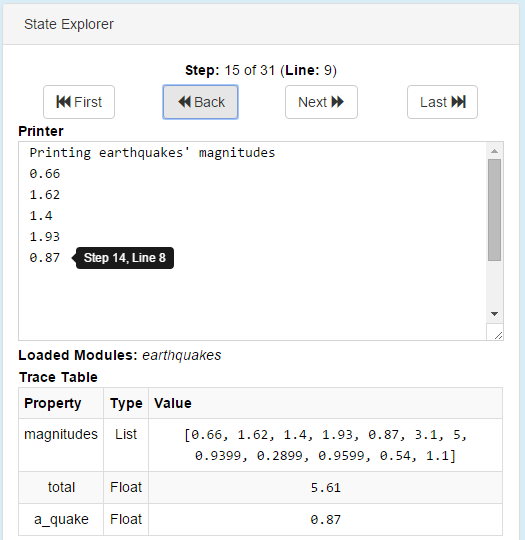
\includegraphics[width=0.4\textwidth]{images/blockpyStateExplorer}
% \end{center}
% \caption{The State Explorer displays information about the entire state of the program, including output and loaded modules.}
% \label{fig-state-explorer}
% \end{figure}

\subsection{State Explorer}

BlockPy provides a State Explorer, used to trace programs' execution over time.
The State Explorer displays more than just information about variables:
Users can step through the code's execution, affecting what is currently printed/plotted, imported modules, and the values and types of variables.

% \begin{figure}
% 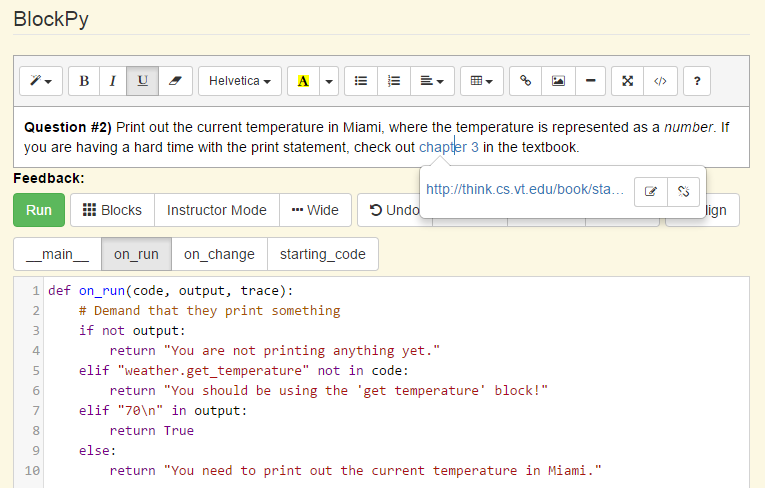
\includegraphics[width=0.5\textwidth]{images/blockpyTeacherEditing}
% \label{fig-teacher-view}
% \caption{Instructor Mode lets you edit questions and and define special functions to give feedback.}
% \end{figure}

\section{Model Use Cases}

In this section, we consider some example scenarios that describe our vision of typical BlockPy use cases.
Our intent is for BlockPy to be useful in both formal and informal situations.

\subsection{Independent Learner}

A learner independently logs into the BlockPy system and selects an introductory problem on calculating averages using iteration: \textit{``Is the weather in Seattle above 60 degrees Fahrenheit? Print Yes or No.''} 
As a complete novice, they are unsure what to do after reading the problem description.
If they decide to cheat by checking the current weather in Seattle and printing the literal value, the system intelligently notices that they are missing a relevant weather block, and explains that they need to combine programmatic decision logic with the appropriate data source.
They think to access the ``Weather'' block category, and grab the \texttt{weather get} block, but are unsure what to do next.
When they run their program, the system notices that they have not used any \texttt{IF} statements, and suggests reading a linked chapter in an online textbook.
If they continue to struggle with integrating pieces, the system can provide increasingly detailed hints until they succeed.

\subsection{Classroom Lesson}

Another common use case for the system would be an instructor with a large classroom of students.
The instructor is using Canvas, an LTI-capable LMS.
They create a series of assignments for the day's classwork.
Students log into Canvas and begin working on the assignments.
As they complete the assignments, their grade is reported to Canvas.
The instructor can monitor progress for the class and check which students are struggling to complete assignments.
This information can allow them to target under-performers with earlier interventions.
The more automatic feedback that instructors make available, the less they need to focus on simple problems (``You were checking the temperature for the wrong city.'') and the more they can focus on students that are truly struggling (``What is iteration?'').

\subsection{1-1 Tutoring}

On several occasions, we have found BlockPy to be a useful tool for correcting individual students' misconceptions.
In particular, the block representation of programs can help beginners grasp that code is not a series of symbols but a structured representation of an algorithm.
Consider a student struggling to write the necessary syntax for indexing a nested dictionary (e.g., a crime report broken into multiple levels, with the burglary rate for a city nested under a violent crime categorization).
The student may not have a clear image of how the layered structure of data can translate into a chain of dictionary accesses.
Sitting with the student, the instructor could build up an expression accessing the data by connecting together dictionary access blocks to the data block, showing the generated Python code at each step.
The learner can visually see how chunks of the code correlate to blocks.

\section{Pilot Study}

BlockPy was piloted in an introductory Computational Thinking course with 35 students in Spring 2015.
These students come from a diverse range of majors, including liberal arts (57\%), architecture (17\%), and sciences (15\%).
There were 20 female students (57\%) and 15 male.
The vast majority of students reported no prior experience in programming, less than 17\% having taken the high school AP course.
Students were evenly distributed across years, with slightly more seniors (29\%), equal percentages of sophomores and juniors (26\%), and fewer freshmen (14\%).

The course content focused on teaching Abstraction and Algorithms.
While programming was not a primary learning objective, was is an important topic in the course for concretely talking about higher level objectives.
The first third of the course, students worked with NetLogo (although they do not program in it, they do read code) and participated in explanatory kinesthetic activities.
Then students were introduced to Python using BlockPy, where they spent roughly six classes on completing guided practice problems.
The next two classes were devoted to using a regular Python environment (Spyder) to complete small programming assignments (similar to the ones done with BlockPy).
Finally, students were given eight class periods to work on an individual final project in Spyder.

\subsection{Methodology}

Student responses to BlockPy were collected through two surveys, one given after the BlockPy section and the other given at the end of the course.
The survey was composed of 4-point Likert questions and open-ended qualitative questions.
A selection of particularly interesting results are shown in Figure~\ref{fig-survey-results}.
All conclusions from this study should be considered preliminary, since it was with the first version of the BlockPy environment.

\subsection{Perceptions of BlockPy}

\begin{figure}
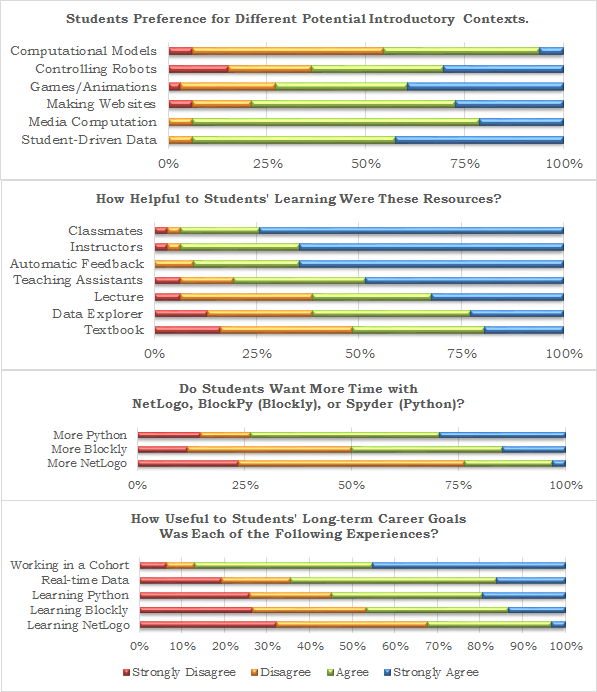
\includegraphics[width=0.5\textwidth]{images/survey-results-smaller}
\caption{Student Responses from Survey on BlockPy}
\label{fig-survey-results}
\end{figure}

% \begin{figure}
% 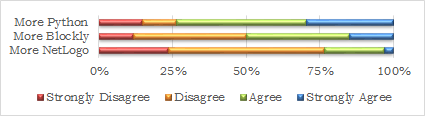
\includegraphics[width=0.5\textwidth]{images/surveyMore-multiColored}
% \caption{Do students want more time with NetLogo, BlockPy (Blockly), or Spyder (Python).}
% \label{fig-want-more}
% \end{figure}

The first survey question asked whether students wanted more time with each of the programming environments they used in the course: NetLogo, BlockPy, or Spyder.
Note that BlockPy was referred to as ``Blockly'', and the Spyder environment was referred to as ``Python''.
These results suggest that students valued their experiences with BlockPy more than NetLogo, but mostly felt that they were not getting enough Python experience. 
This is backed up by the qualitative data, where some students say ``More Blockly, Less Python'', but others ask for ``More Blockly and More Python''.

\subsection{Usage of BlockPy}

Over the six days spent using BlockPy, students were tasked with 40 classwork questions and 19 homework questions.
Students ran their code an average of 4 times per problem (standard deviation 1.8).

Students were asked if they felt successful in the transition from BlockPy to Spyder.
Only 65\% of the class agreed or strongly agreed, suggesting that there was a sizeable population that felt uncomfortable during that transition.
The original design of the mutual language translation featured the block and text view simultaneously, side-by-side.
However, analysis of the logs reveals that most students did not take advantage of the feature.
Only 5 students (roughly 15\%) had used the conversion functionality at all, and fewer used it consistently.
It is possible that students were observing the code as it changed, but they were not writing textual code.
It is difficult to say why exactly students did not take advantage of it.
Our current hypothesis is that students were confused by the interface, which required manual conversion to go from text to blocks.
In our new version, the conversion happens automatically, simply by switching tabs, and we provide intentional opportunities for the students to switch.
Preliminary data suggests this new interface greatly improves students' transition.

% \begin{figure}
% 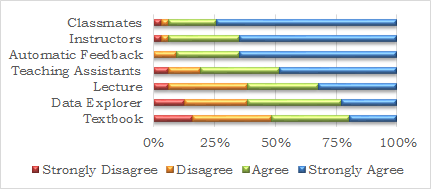
\includegraphics[width=0.5\textwidth]{images/surveyHelpfulness-multiColored}
% \caption{How helpful to students' learning were these resources?}
% \label{fig-survey-helpfulness}
% \end{figure}

Students were surveyed about what helped their learning the most.
Peer learning and instructors were about on par with the automatic feedback given in BlockPy, suggesting the strong value of the system.
Despite the popular response to the State Explorer, relatively few students took advantage of it (11 students, roughly 31\%).
Since more than 50\% of the class reported finding value in the data explorer, it is possible that the students benefited from instructor presentations of the tool, even if they didn't take advantage of it themselves. 

% \begin{figure}
% 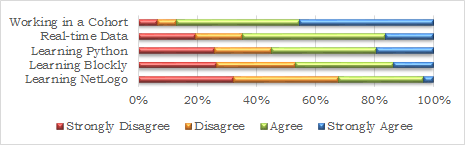
\includegraphics[width=0.5\textwidth]{images/surveyUsefulness-multiColored}
% \caption{How useful to students' long-term career goals was each of the following experiences?}
% \label{fig-survey-usefulness}
% \end{figure}

% \begin{figure}
% 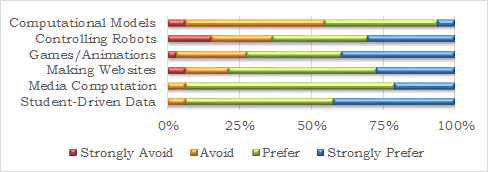
\includegraphics[width=0.5\textwidth]{images/surveyContexts-multiColored}
% \caption{Students preference for different potential introductory contexts.}
% \label{fig-survey-context}
% \end{figure}

\subsection{Data Science Context}

Students were surveyed about their perceptions of the value of different course experiences with regards to their long-term career goals and their interest in potential contexts for introductory computing courses.
Each of these contexts were briefly described -- for example, the Media Comp context was listed as ``working with pictures, sounds and movies.''
Both sets of results suggest that students find data science to be compelling, but this should be taken with a grain of salt, since students have negligible experience with alternative contexts.
However, our preliminary results suggest that this is an approach worth exploring further.

\section{Future Work}

BlockPy is an evolving project.
We have a number of features planned to expand Python support.
We are also planning on expanding support for the guided feedback API for instructors, such as leveraging more static/dynamic type inference techniques to improve block rendering and error reporting.

We also have research questions posed by the block-based nature of the interface.
One of the biggest values of a block-based environment is that it can immediately expose the breadth of a rich API.
This greatly reduces students' dependency on documentation.
Of course, exposing this breadth can also be a downside, as students might be overwhelmed by the features in the interface.
It is an open research question to decide what rate to expose language features.

One of the major advantages of game and animation design as an introductory context is that they make abstract concepts concrete. 
Further analysis is needed to determine the trade-offs of using different contexts.
BlockPy can support this by supporting these alternative contexts, such as turtle graphics and media computation libraries.

It is difficult to derive conclusive results from our pilot due to the small population size and the evolving nature of BlockPy.
Preliminary results from more in-progress studies suggest that recent improvements have overcome a number of limitations to the environment and user feedback has dramatically improved.
We are conducting follow-up studies on the logged students' code, even as we collect more data on the newest iteration.
We are hopeful that BlockPy will increase its user base, providing a larger sample of learners to conduct research on, and provide more meaningful data.

\subsection{Missing Language features}

BlockPy is being developed in an on-demand fashion, driven by immediate  course needs, but is still limited.
For example, the block interface does not support a number of advanced Python features, such as an interface for writing Object-oriented classes.
This does not mean that students cannot write programs featuring classes or other advanced features.
Python code using these features will render in BlockPy as embedded text blocks and will execute through Skulpt normally.
There is no technical impediment to supporting these features, the process is limited only by time and community interest.


\section{Conclusion}

In this paper, we have introduced BlockPy, our block-based environment for Python.
It is open-source and available for use for free at \url{http://www.blockpy.com/}.
We believe that BlockPy represents a new paradigm for introductory learners, blending interactive support with a strong path to programming maturity.
By teaching in the context of data science, we provide authenticity even as we move students out of the system towards a more serious environment. 
Research with BlockPy will help answer crucial questions about the value of data science and blocks.
Our hope is that BlockPy's open nature can encourage learners from diverse fields to engage with computing in a way that will lead to a computing-rich future for a larger population.

% An example of a floating figure using the graphicx package.
% Note that \label must occur AFTER (or within) \caption.
% For figures, \caption should occur after the \includegraphics.
% Note that IEEEtran v1.7 and later has special internal code that
% is designed to preserve the operation of \label within \caption
% even when the captionsoff option is in effect. However, because
% of issues like this, it may be the safest practice to put all your
% \label just after \caption rather than within \caption{}.
%
% Reminder: the "draftcls" or "draftclsnofoot", not "draft", class
% option should be used if it is desired that the figures are to be
% displayed while in draft mode.
%
%\begin{figure}[!t]
%\centering
%\includegraphics[width=2.5in]{myfigure}
% where an .eps filename suffix will be assumed under latex, 
% and a .pdf suffix will be assumed for pdflatex; or what has been declared
% via \DeclareGraphicsExtensions.
%\caption{Simulation results for the network.}
%\label{fig_sim}
%\end{figure}

% Note that the IEEE typically puts floats only at the top, even when this
% results in a large percentage of a column being occupied by floats.


% An example of a double column floating figure using two subfigures.
% (The subfig.sty package must be loaded for this to work.)
% The subfigure \label commands are set within each subfloat command,
% and the \label for the overall figure must come after \caption.
% \hfil is used as a separator to get equal spacing.
% Watch out that the combined width of all the subfigures on a 
% line do not exceed the text width or a line break will occur.
%
%\begin{figure*}[!t]
%\centering
%\subfloat[Case I]{\includegraphics[width=2.5in]{box}%
%\label{fig_first_case}}
%\hfil
%\subfloat[Case II]{\includegraphics[width=2.5in]{box}%
%\label{fig_second_case}}
%\caption{Simulation results for the network.}
%\label{fig_sim}
%\end{figure*}
%
% Note that often IEEE papers with subfigures do not employ subfigure
% captions (using the optional argument to \subfloat[]), but instead will
% reference/describe all of them (a), (b), etc., within the main caption.
% Be aware that for subfig.sty to generate the (a), (b), etc., subfigure
% labels, the optional argument to \subfloat must be present. If a
% subcaption is not desired, just leave its contents blank,
% e.g., \subfloat[].


% An example of a floating table. Note that, for IEEE style tables, the
% \caption command should come BEFORE the table and, given that table
% captions serve much like titles, are usually capitalized except for words
% such as a, an, and, as, at, but, by, for, in, nor, of, on, or, the, to
% and up, which are usually not capitalized unless they are the first or
% last word of the caption. Table text will default to \footnotesize as
% the IEEE normally uses this smaller font for tables.
% The \label must come after \caption as always.
%
%\begin{table}[!t]
%% increase table row spacing, adjust to taste
%\renewcommand{\arraystretch}{1.3}
% if using array.sty, it might be a good idea to tweak the value of
% \extrarowheight as needed to properly center the text within the cells
%\caption{An Example of a Table}
%\label{table_example}
%\centering
%% Some packages, such as MDW tools, offer better commands for making tables
%% than the plain LaTeX2e tabular which is used here.
%\begin{tabular}{|c||c|}
%\hline
%One & Two\\
%\hline
%Three & Four\\
%\hline
%\end{tabular}
%\end{table}


% Note that the IEEE does not put floats in the very first column
% - or typically anywhere on the first page for that matter. Also,
% in-text middle ("here") positioning is typically not used, but it
% is allowed and encouraged for Computer Society conferences (but
% not Computer Society journals). Most IEEE journals/conferences use
% top floats exclusively. 
% Note that, LaTeX2e, unlike IEEE journals/conferences, places
% footnotes above bottom floats. This can be corrected via the
% \fnbelowfloat command of the stfloats package.





% conference papers do not normally have an appendix


% use section* for acknowledgment
\section*{Acknowledgments}

We gratefully acknowledge the support of the National Science Foundation under Grants DGE-0822220, DUE-1444094, and DUE-1624320.




\bibliographystyle{IEEEtran}
\bibliography{references}
\addbibresource{./references.bib}
\printbibliography

\begin{IEEEbiography}[{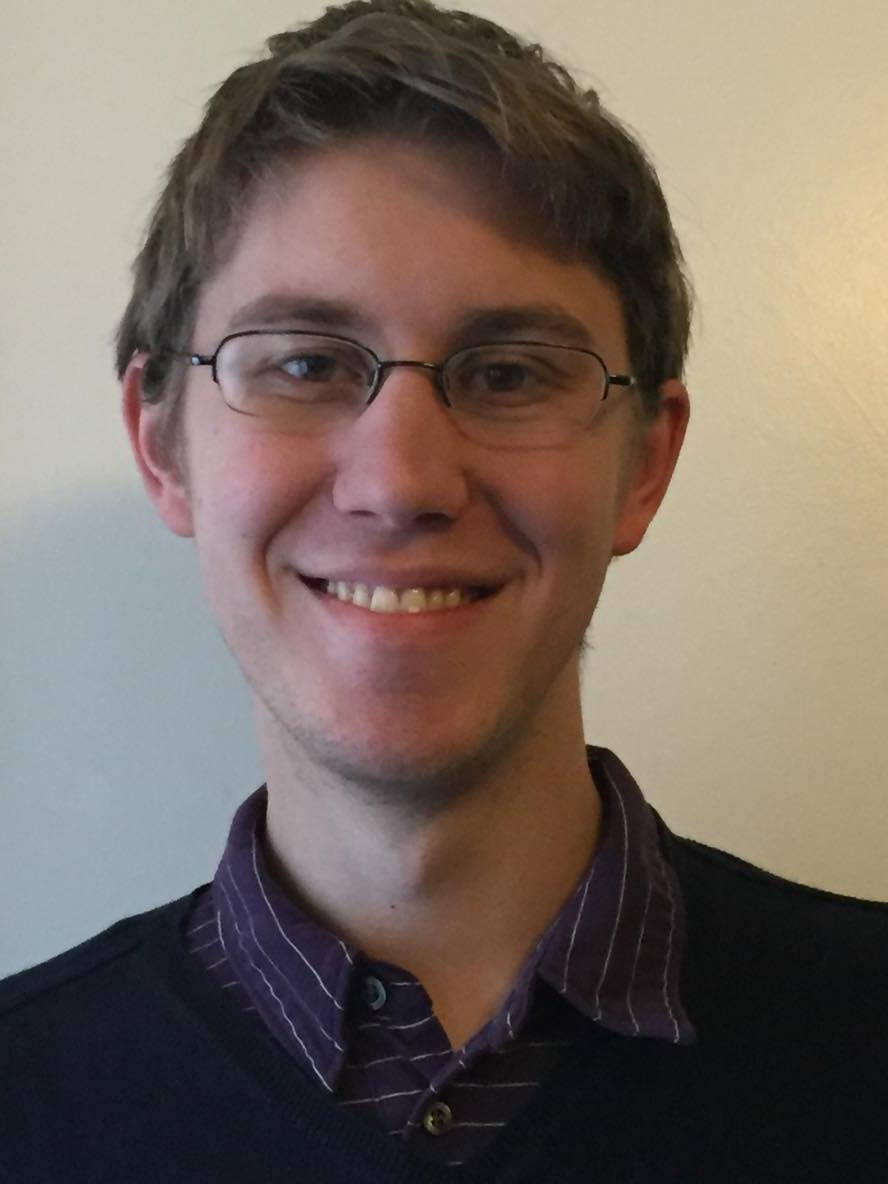
\includegraphics[width=1in,height=1.25in,clip,keepaspectratio]{biography/bart}}]{Austin Cory Bart}
is a PhD candidate at Virginia Tech studying Computer Science and Learning Sciences. He received his undergraduate degree from the University of Delaware in Computer Science. His research interests are Computer Science Education, Software Engineering, and Program Analysis.
\end{IEEEbiography}

\begin{IEEEbiography}[{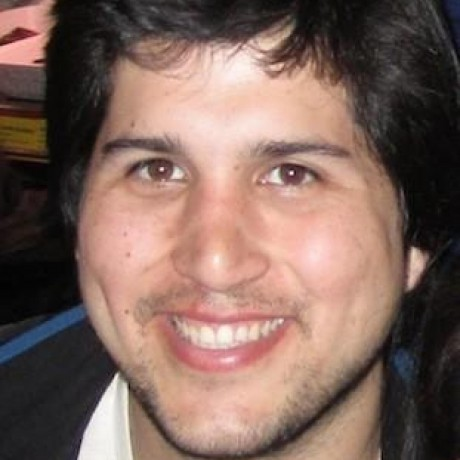
\includegraphics[width=1in,height=1.25in,clip,keepaspectratio]{biography/tibau}}]{Javier Tibau}
is a PhD candidate at Virginia Tech studying Computer Science. He has an undergraduate degree from Escuela Superior Politecnica del Litoral (ESPOL), and a MSc from Universitat Politecnica de Catalunya. His research interests are in Human-Computer Interaction, and Computer Science Education.
\end{IEEEbiography}

\begin{IEEEbiography}[{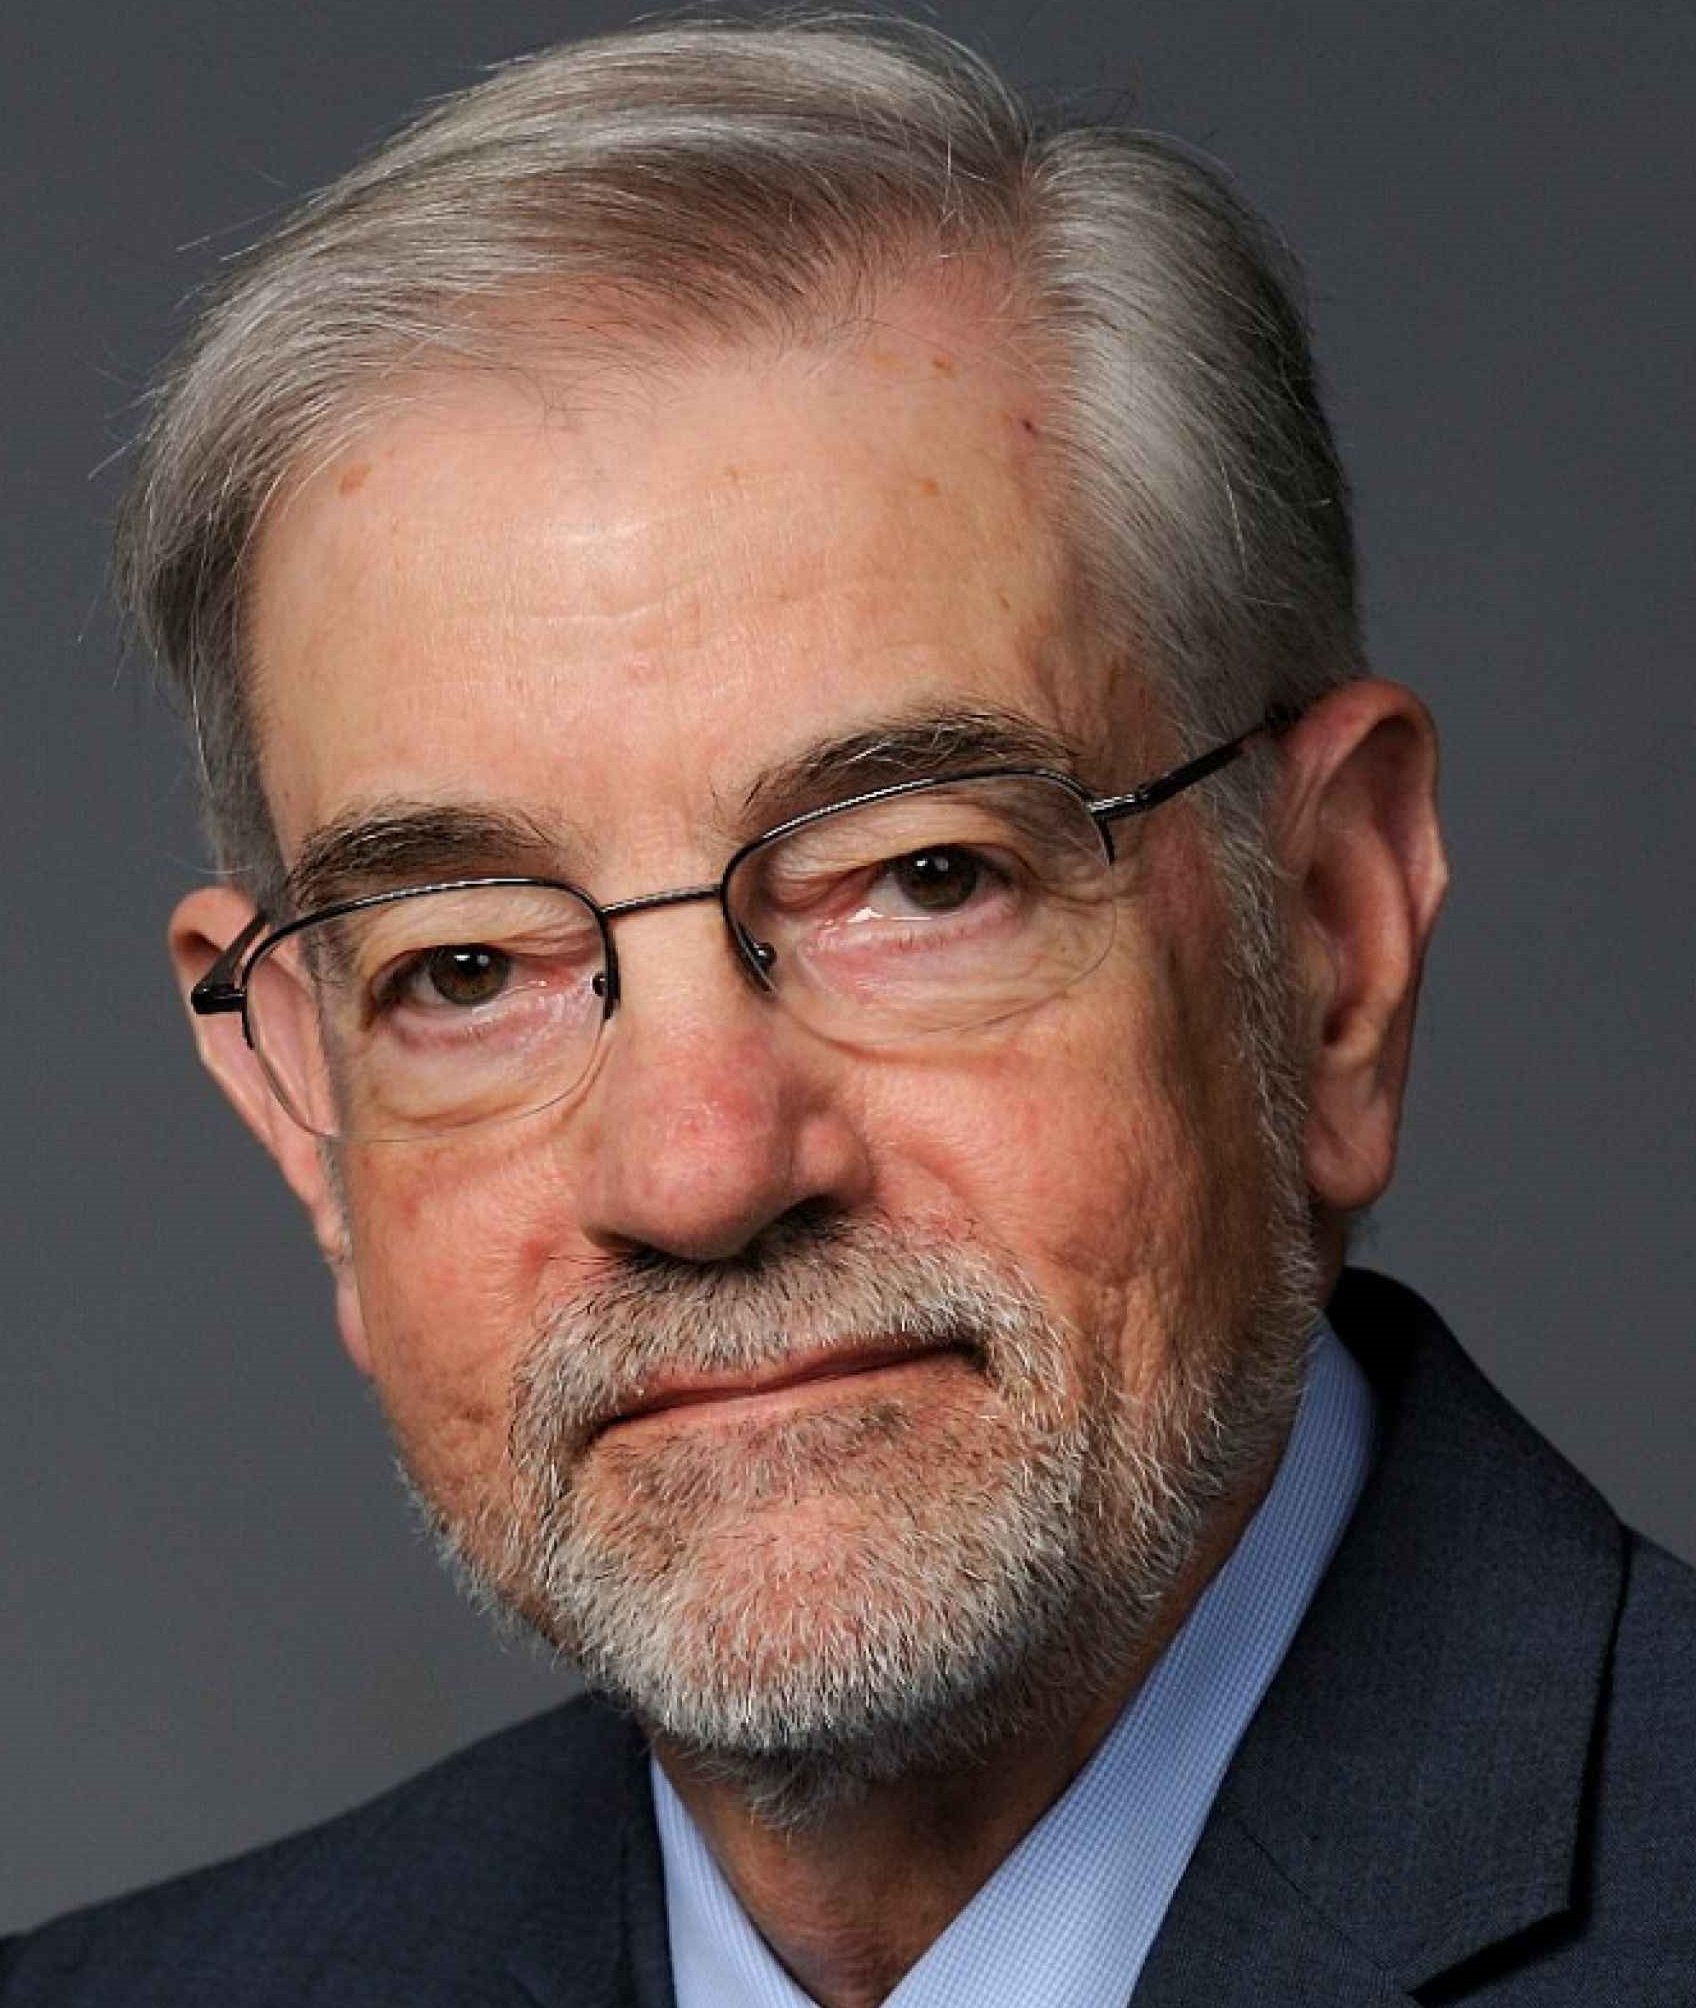
\includegraphics[width=1in,height=1.25in,clip,keepaspectratio]{biography/kafura}}]{Dennis Kafura}
received his PhD from Purdue University. He is a Professor of Computer Science at Virginia Tech. He is the PI on two NSF IUSE awards both of which involved the development of a general education course in Computational Thinking at the university level using the BlockPy environment.
\end{IEEEbiography}

\begin{IEEEbiography}[{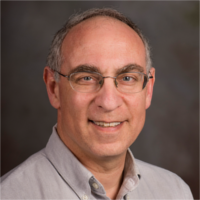
\includegraphics[width=1in,height=1.25in,clip,keepaspectratio]{biography/shaffer}}]{Clifford A. Shaffer} (Senior Member, IEEE and Distinguished Member, ACM) received his PhD from the University of Maryland.
He is Professor of Computer Science at Virginia Tech.
His current research interests are in Computational Biology (specifically, user interfaces for specifying models and computations), Algorithm Visualization, and Computer Science Education.

\end{IEEEbiography}

\begin{IEEEbiography}[{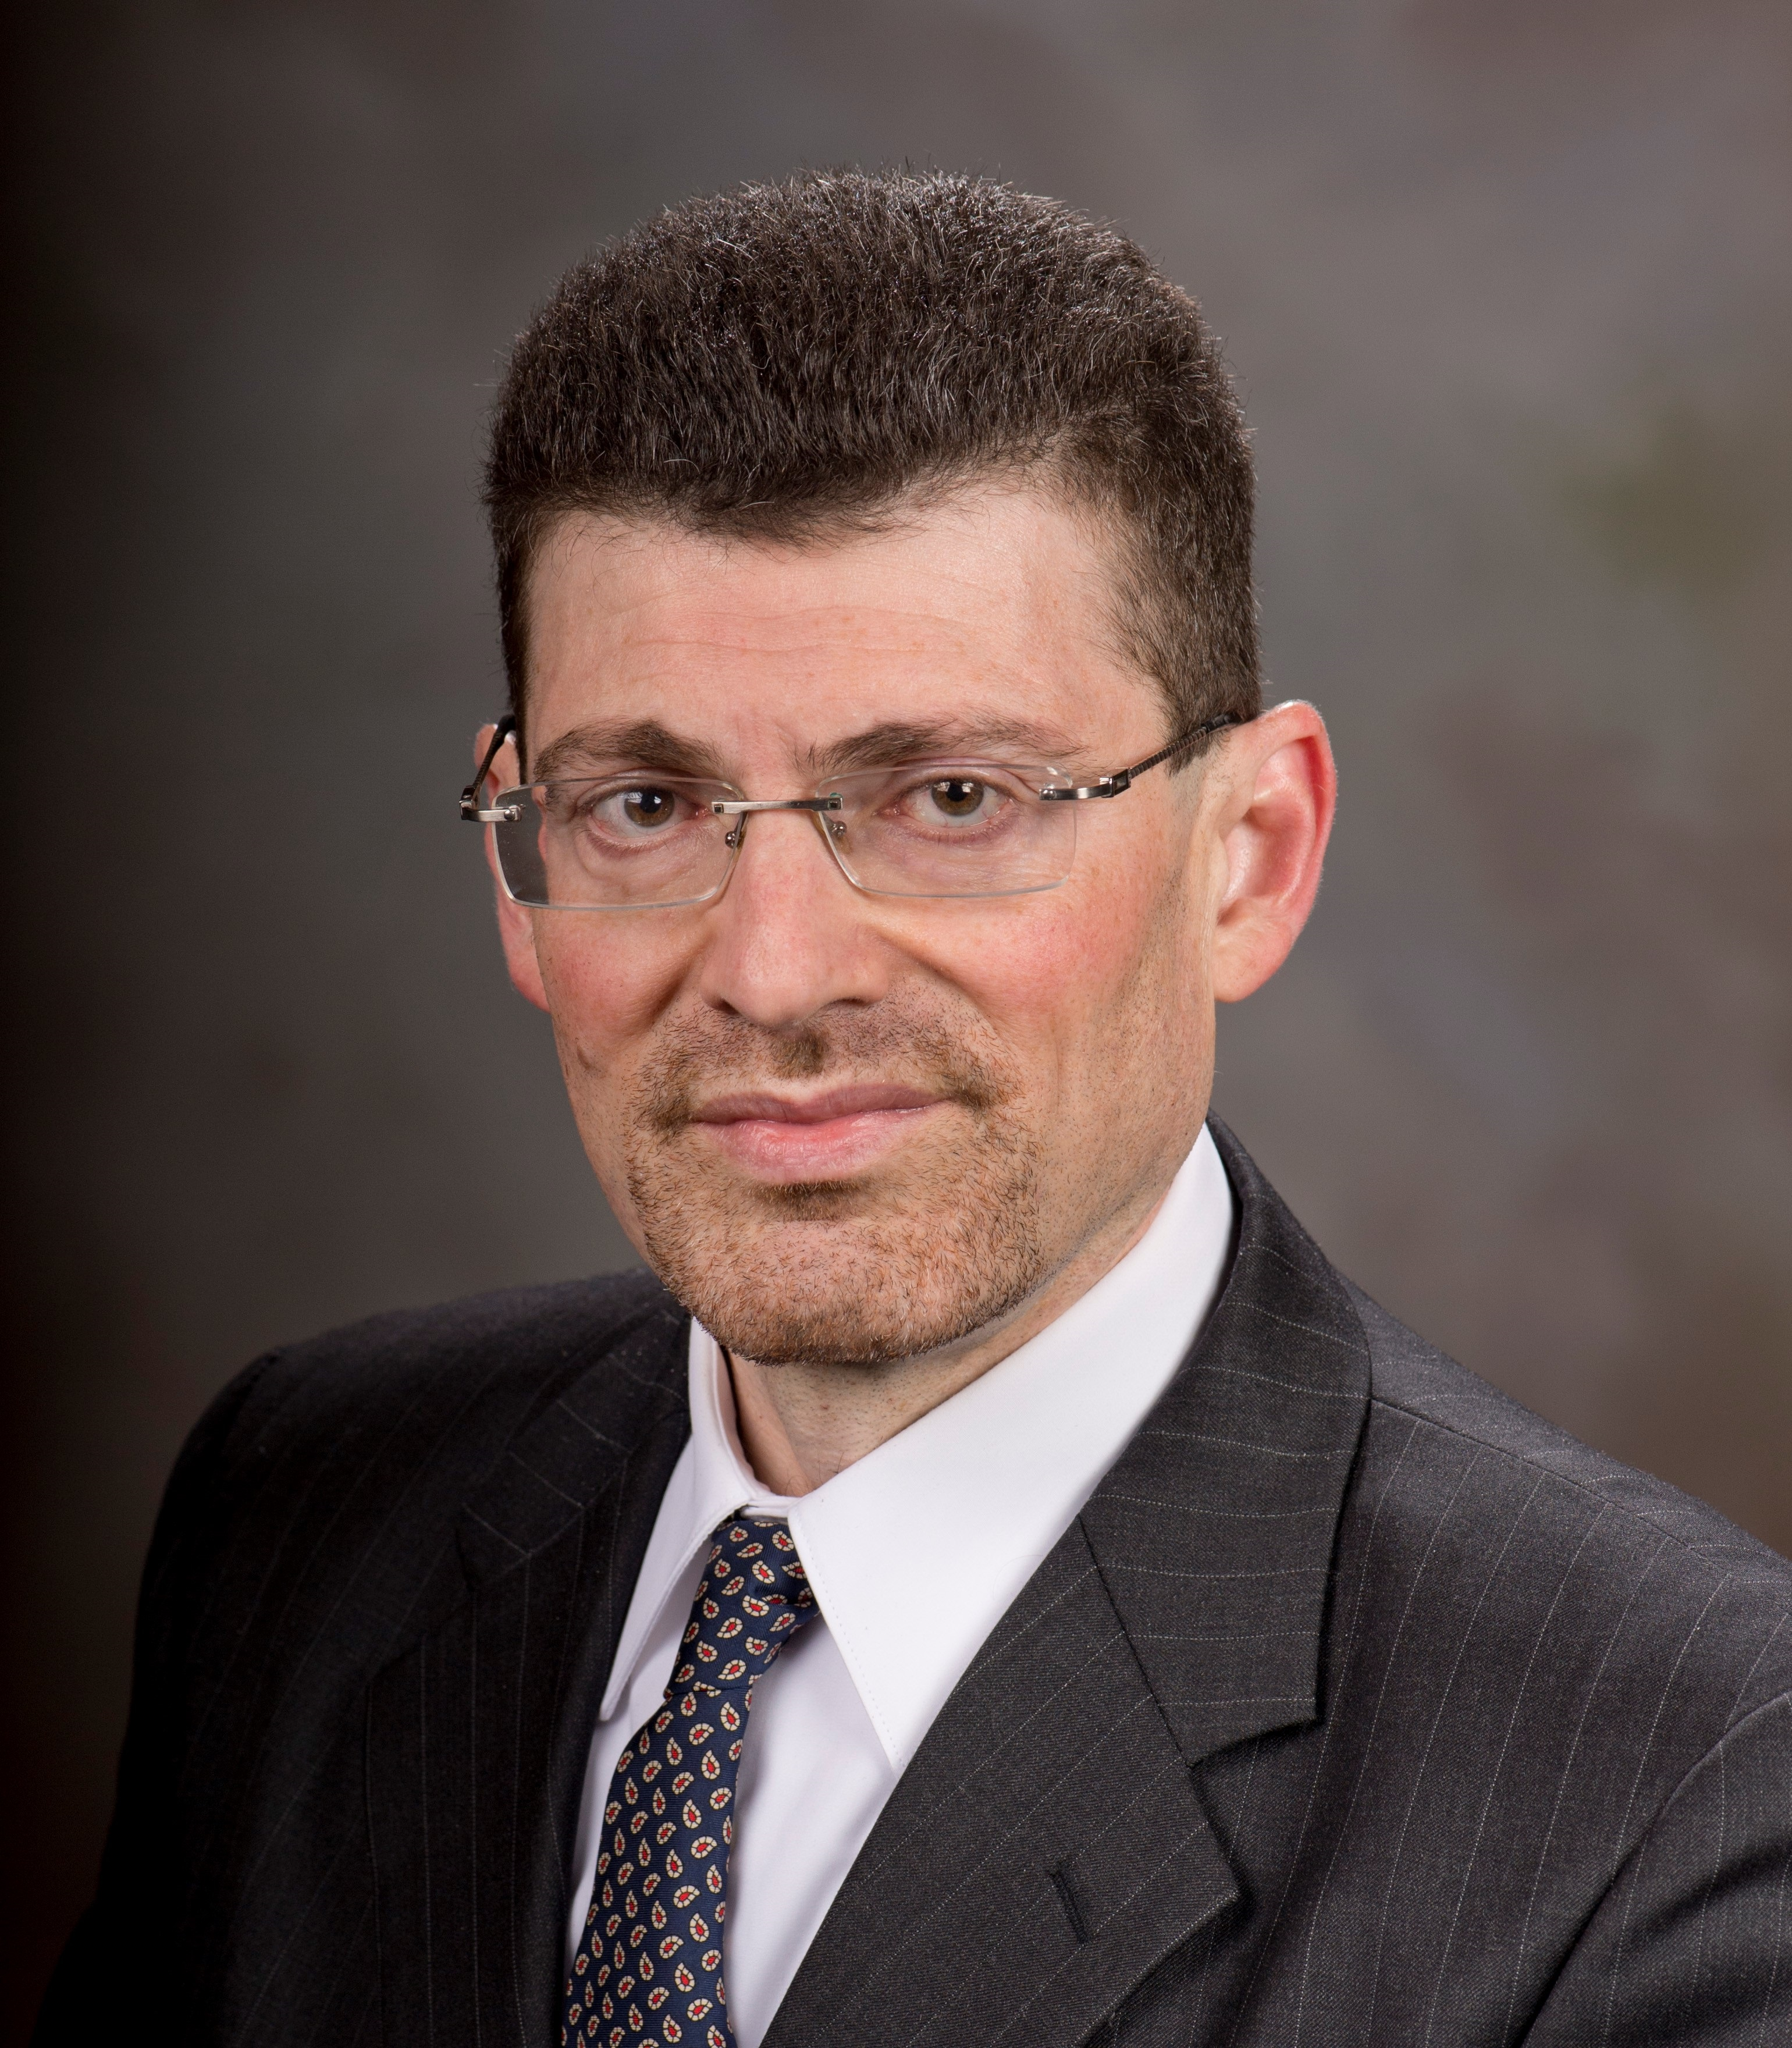
\includegraphics[width=1in,height=1.25in,clip,keepaspectratio]{biography/tilevich}}]{Eli Tilevich}(Senior Member, IEEE) received his PhD from Georgia Tech.
He is an Associate Professor of Computer Science at Virginia Tech. His recent publications and current research focus on Software Engineering for Distributed and Mobile Computing and on Computer Science Education.
\end{IEEEbiography}


% that's all folks
\end{document}


